\section{Conclusion}

\begin{refsection}
\begin{frame}{Takeaways and Thank Yous}

\vspace{-1em}

\begin{itemize}
	\item \#SAT solvers effectively tackle quantum compilation problems
%	\item Better data structures yield better circuit simulation, equivalence checks \& synthesis
	\item \limdd unites the strengths of decision diagrams and the stabilizer formalism
	\item \limdd, MPS and RBM are incomparable in terms of succinctness
	\item Rapidity tells us that MPS and \limdd are never much slower than QMDD, ADD
\end{itemize}


\vspace{2em}

\pause

%\includegraphics[height=2cm]{graphics/thanos.jpg}
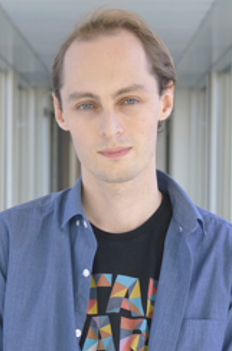
\includegraphics[height=2cm]{graphics/brand.png}
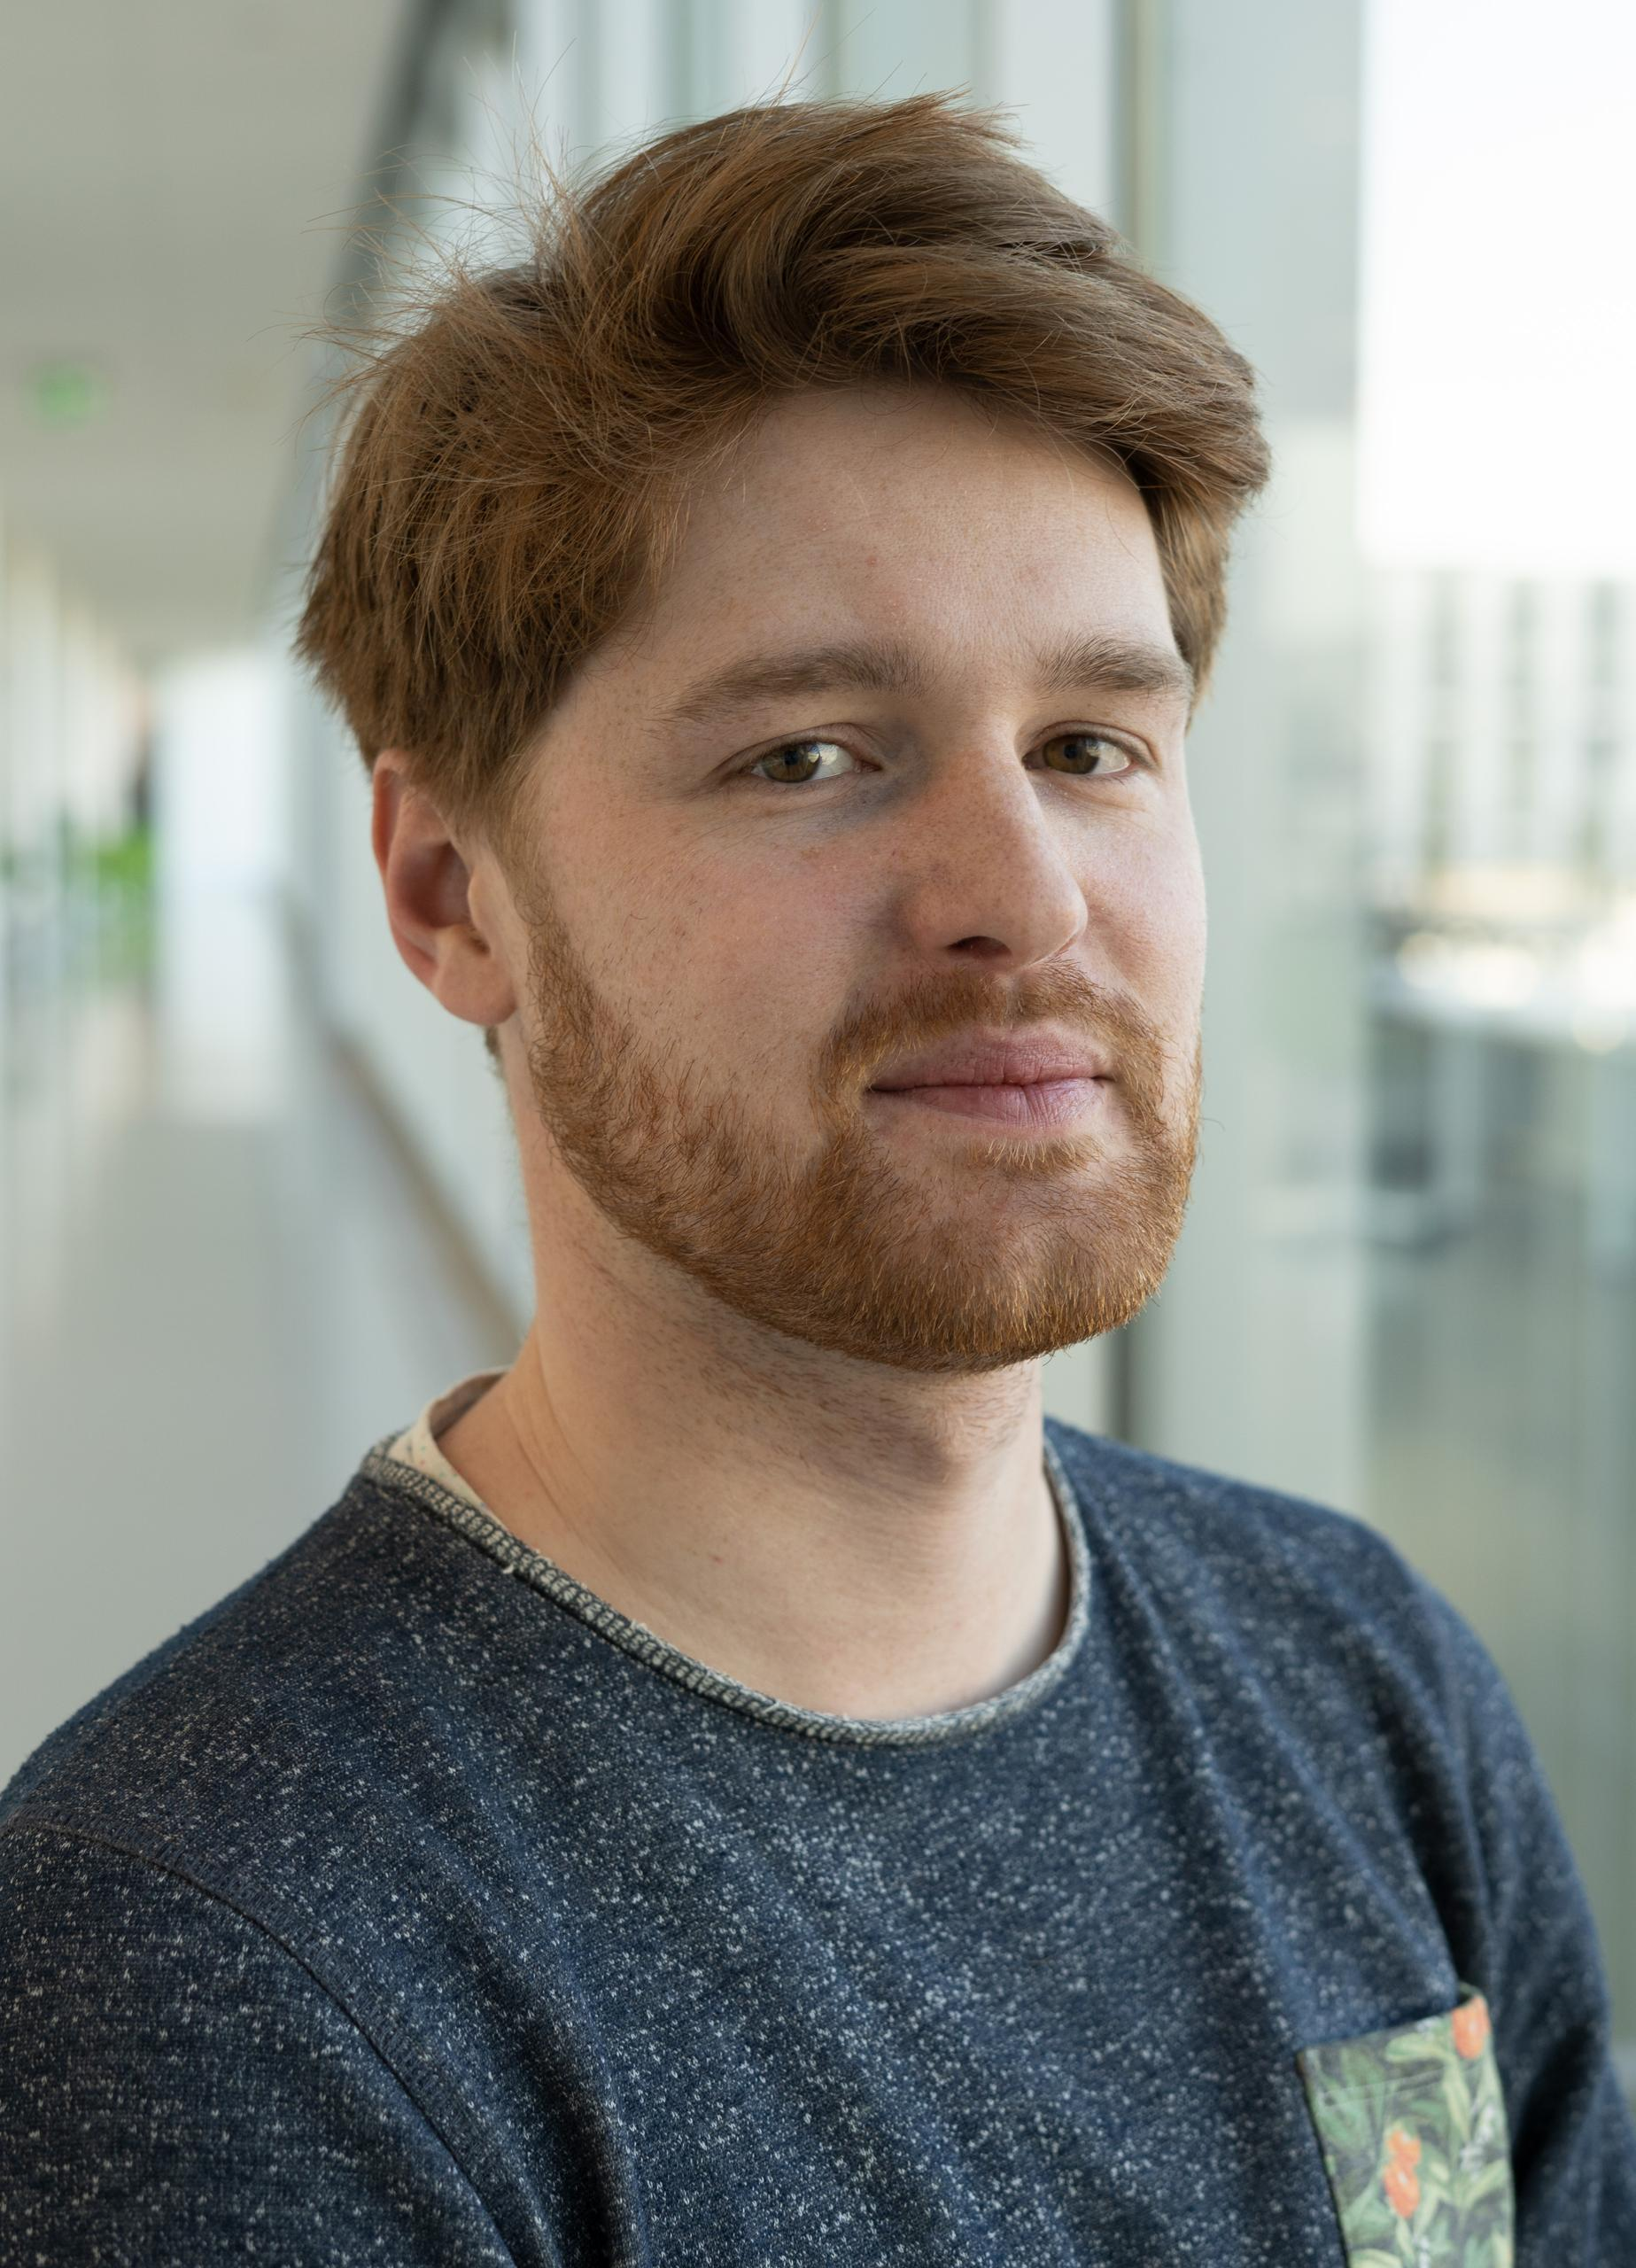
\includegraphics[height=2cm]{graphics/coopmans_tim}
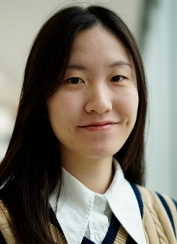
\includegraphics[height=2cm]{graphics/mei.png}
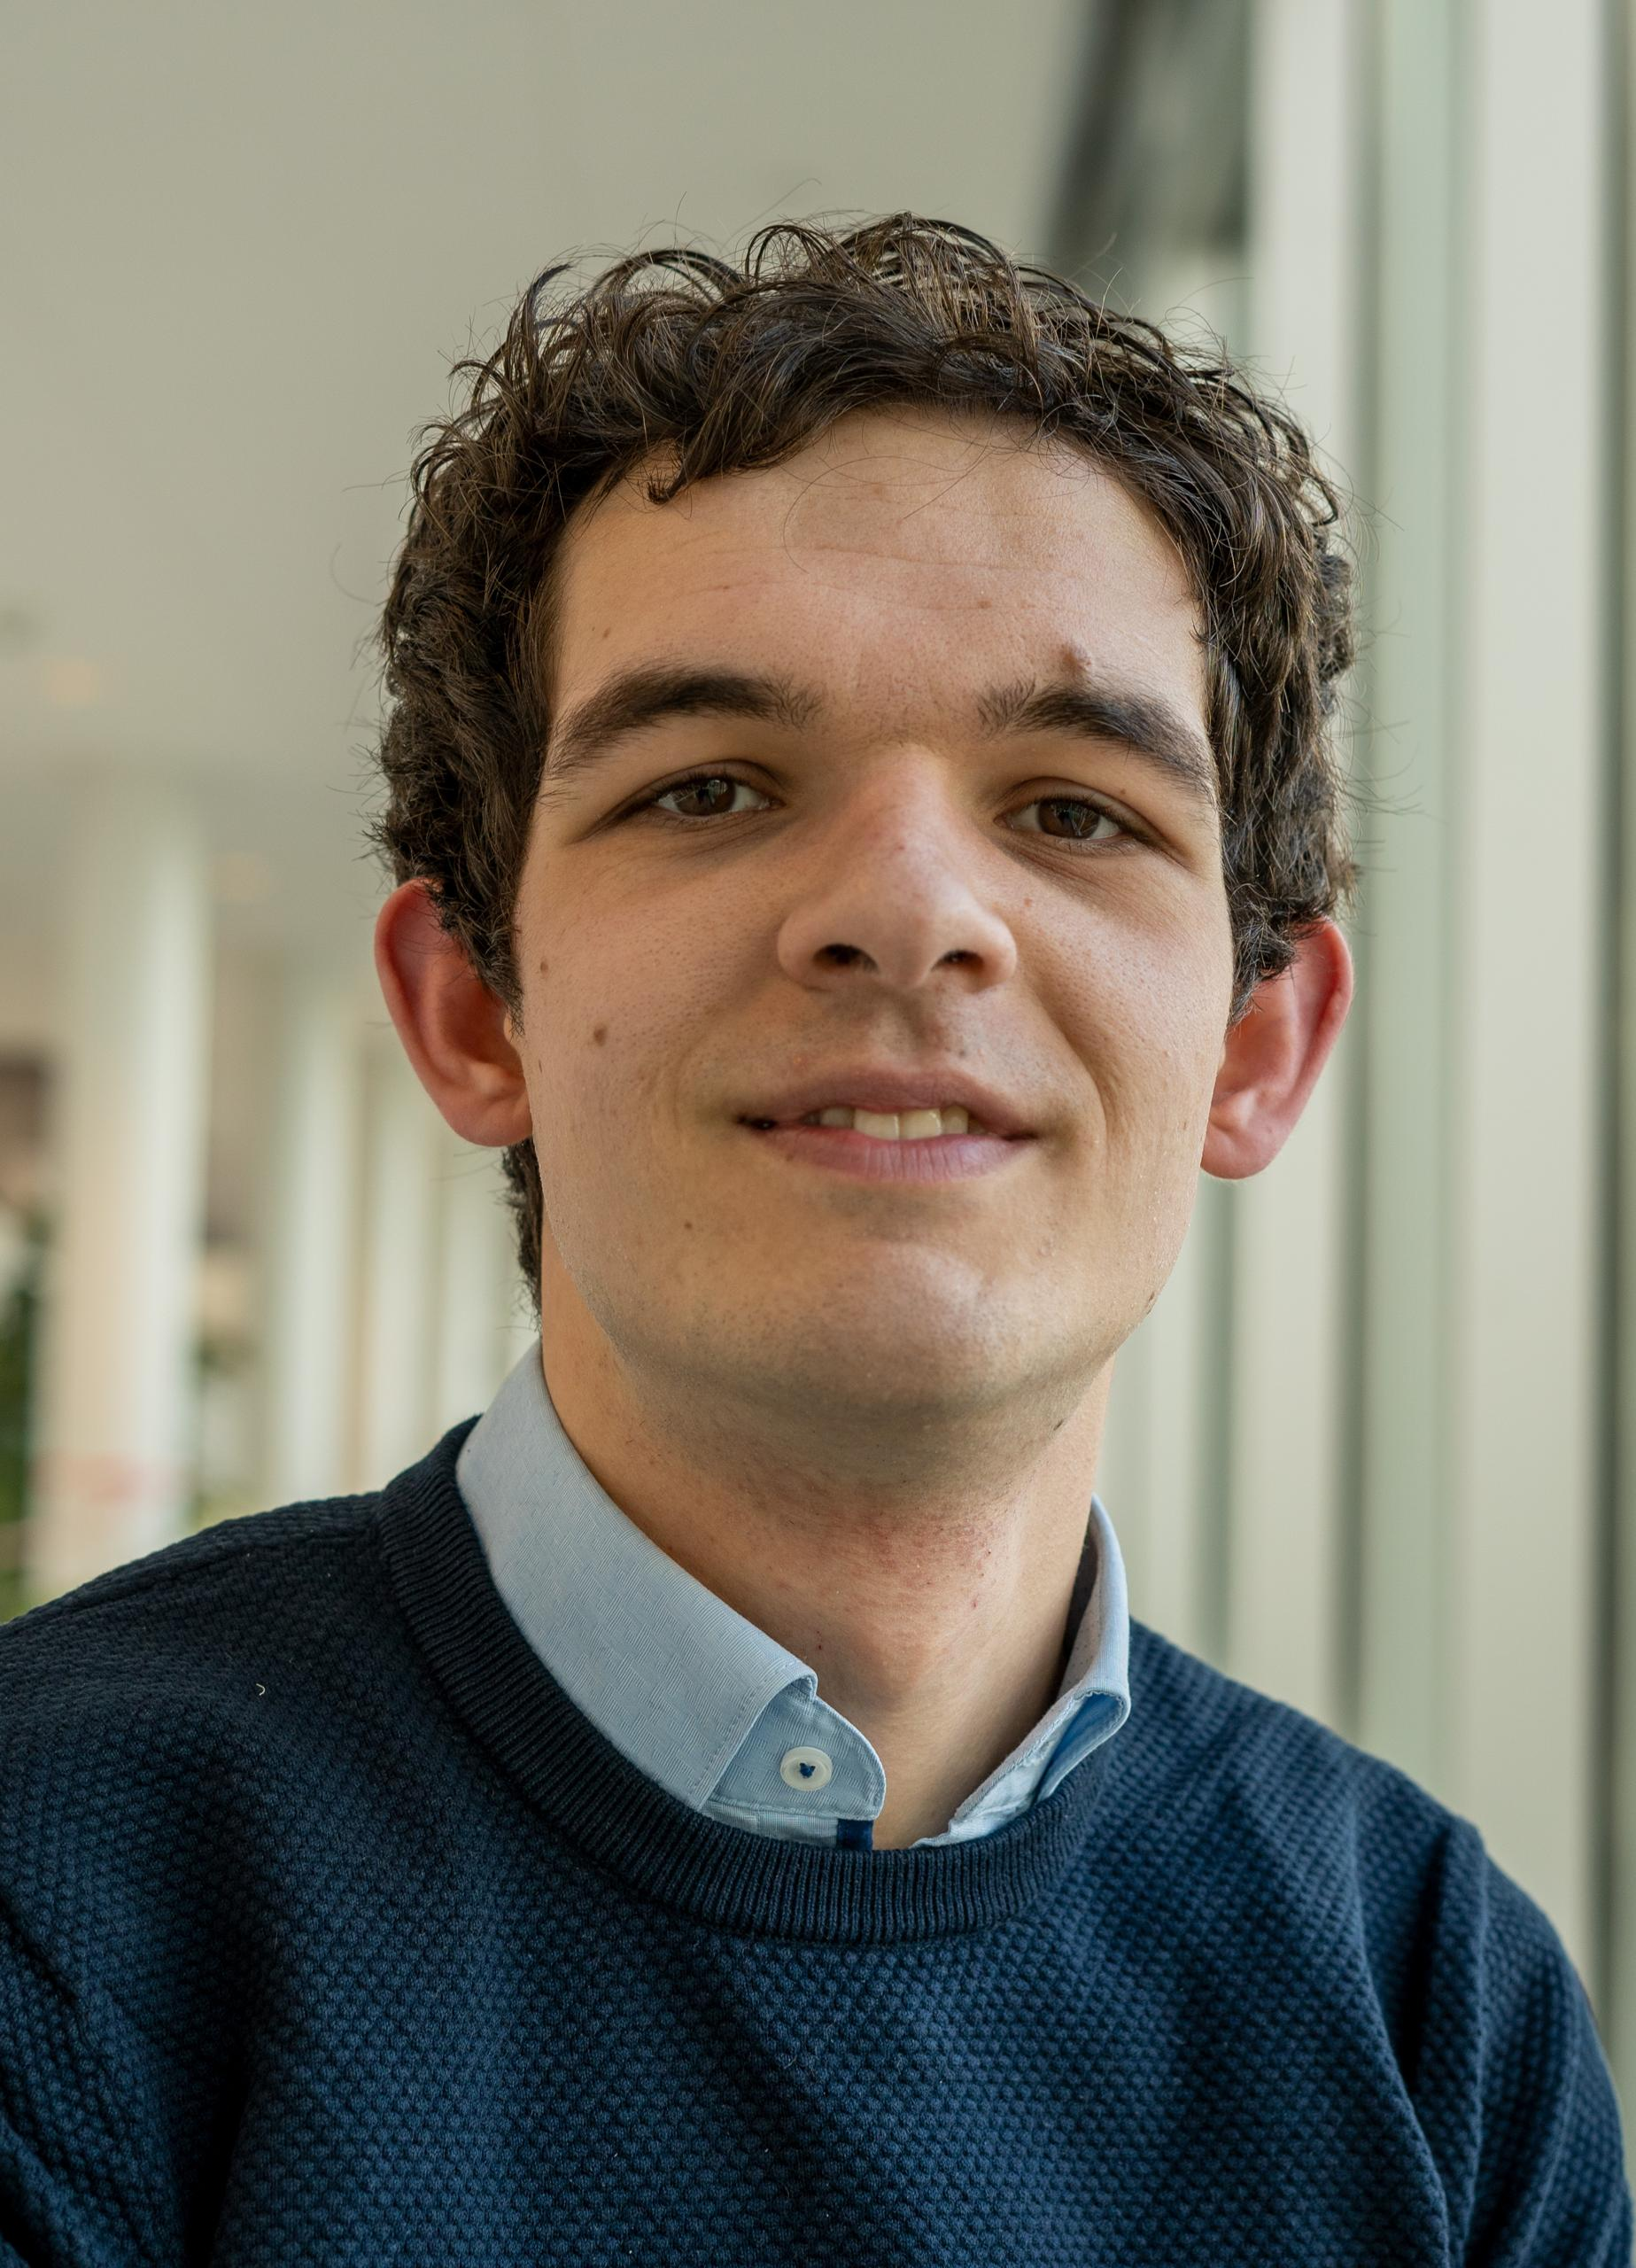
\includegraphics[height=2cm]{graphics/quist_arend-jan.jpg}
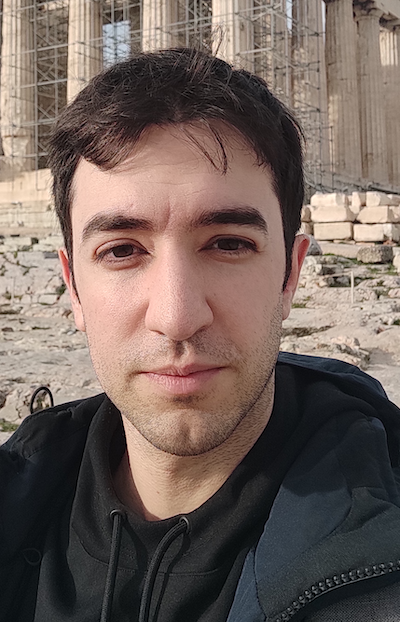
\includegraphics[height=2cm]{graphics/dimitrios}
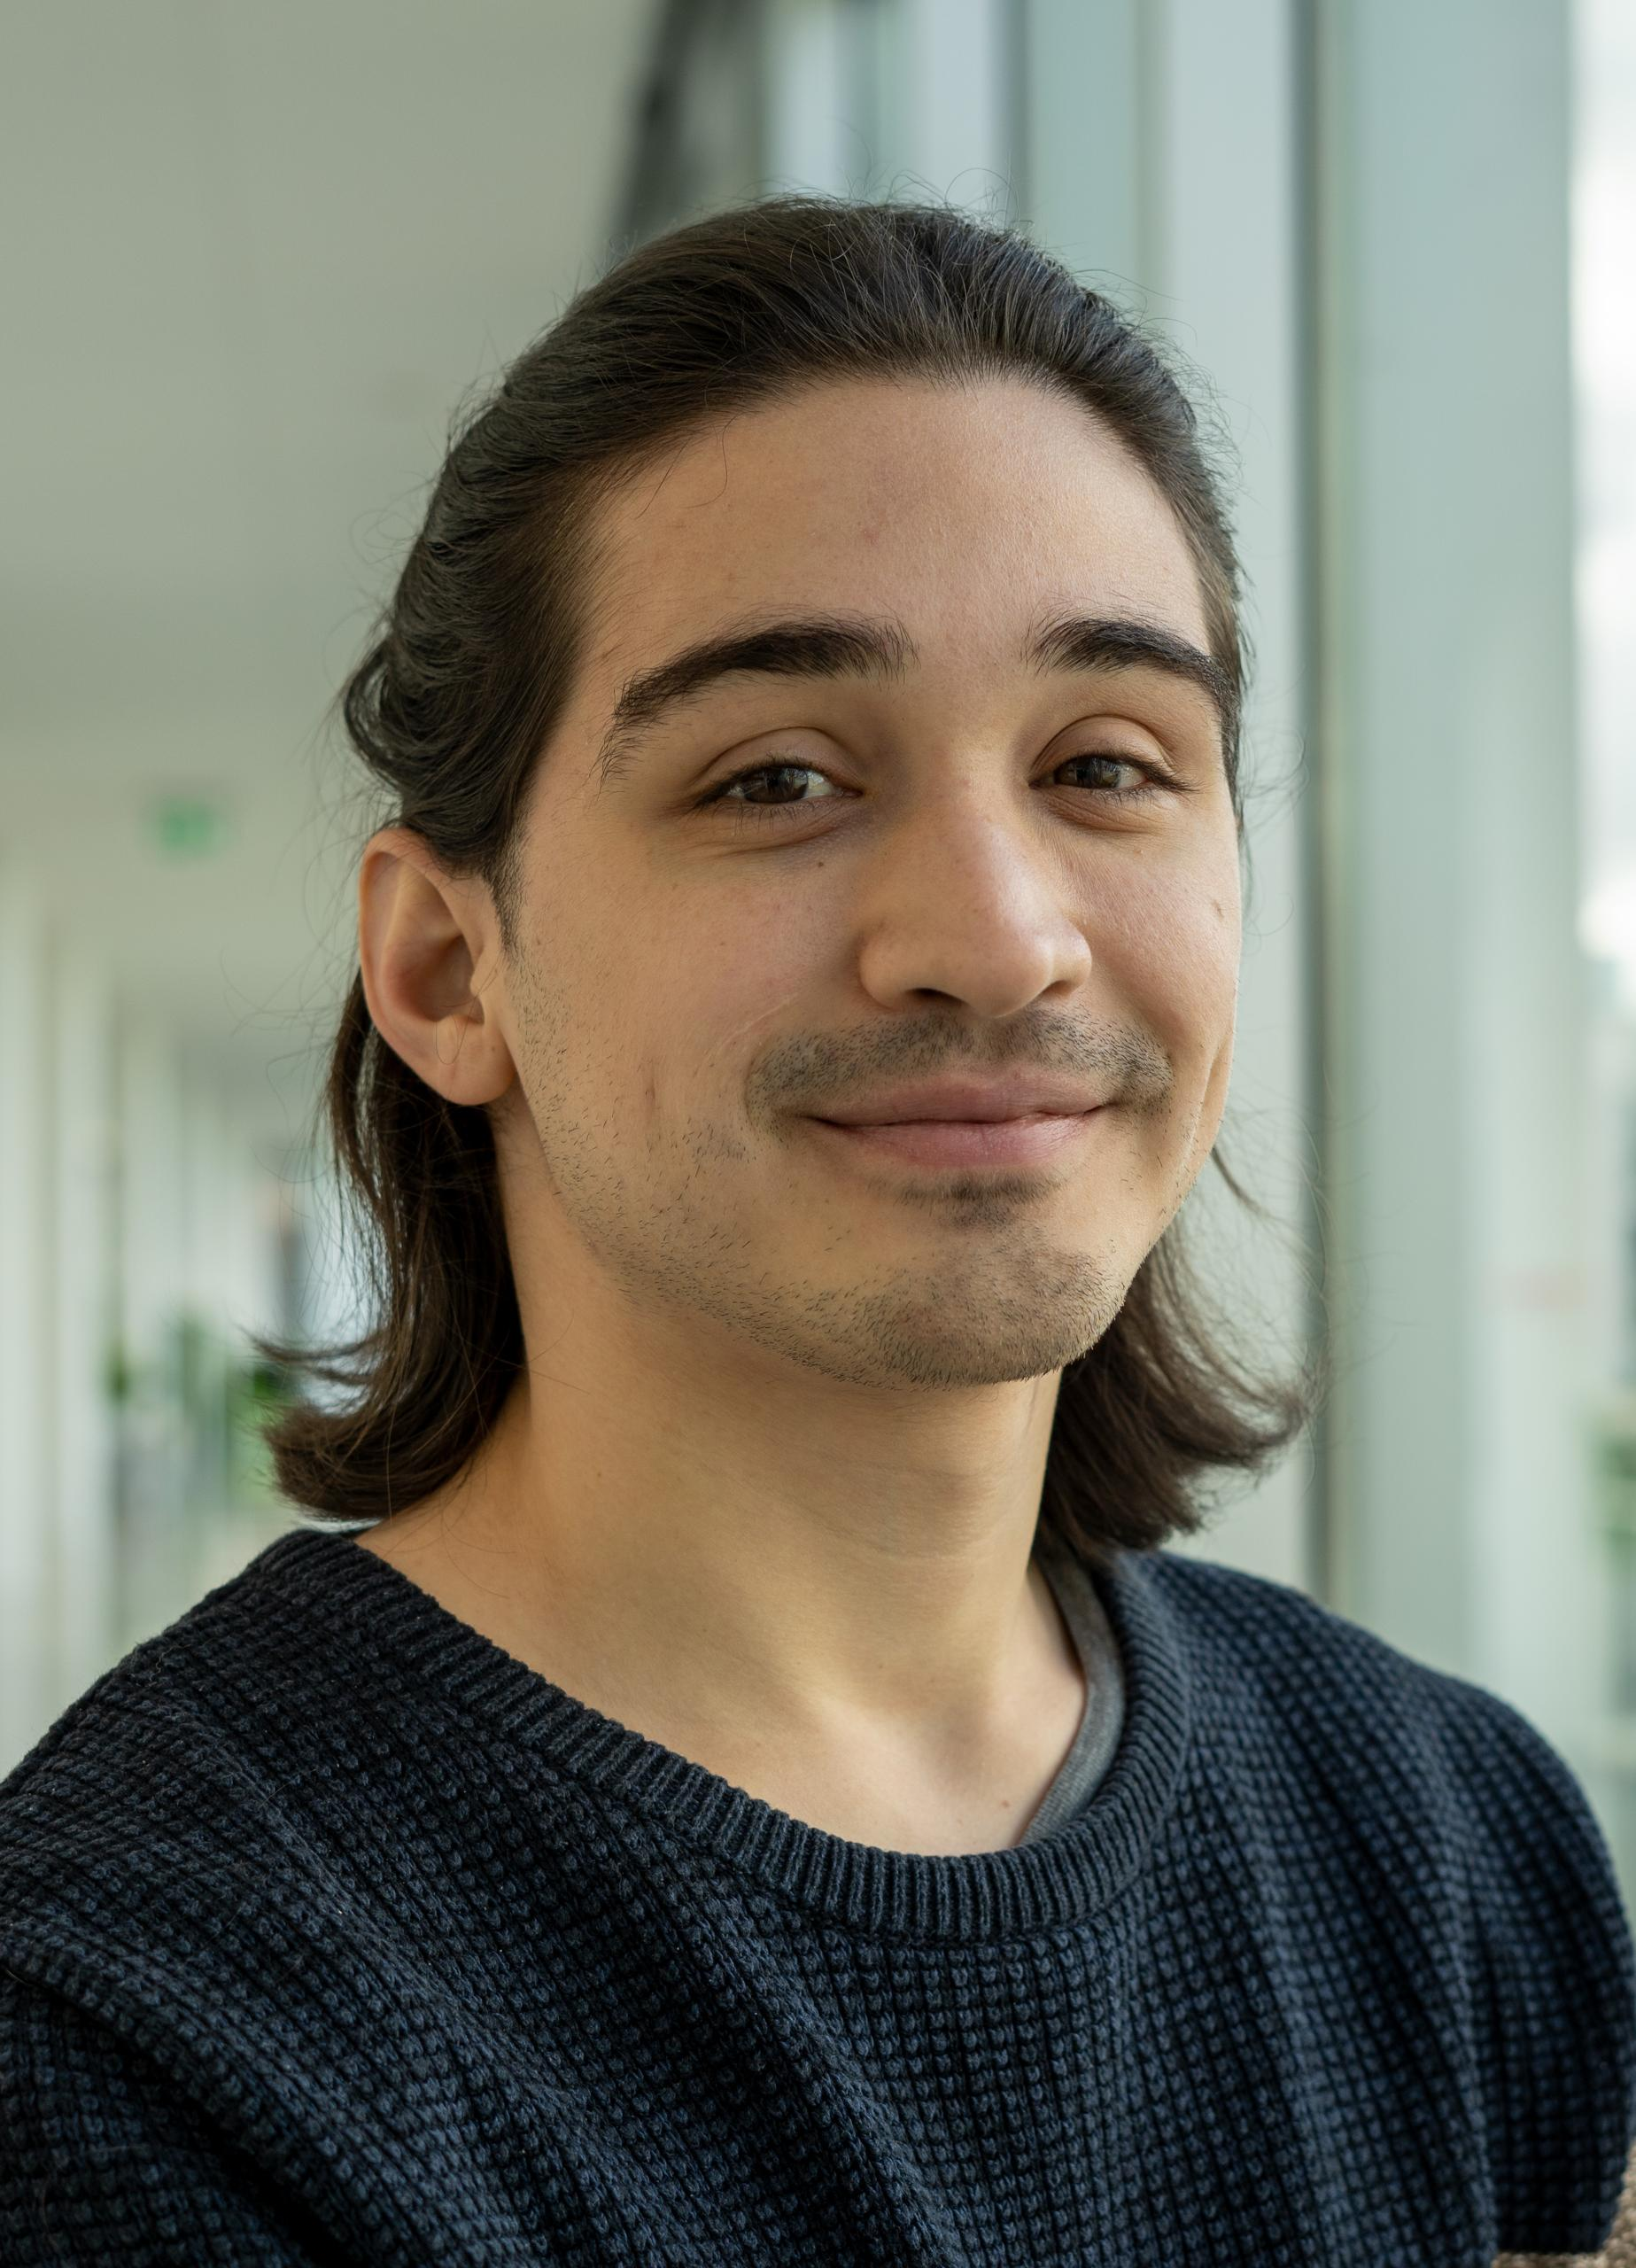
\includegraphics[height=2cm]{graphics/villoria_alejandro.jpg}
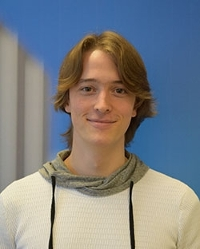
\includegraphics[height=2cm]{graphics/lieuwe.jpeg}
%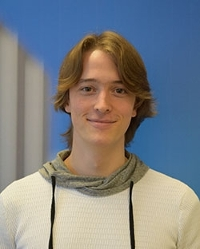
\includegraphics[width=2cm]{graphics/lieuwe}

\footnotesize
Sebastiaan Brand~~~~~~~~~~~~~~~~~~~
Jingyi Mei~~~~~~~~~~~~~~~~~~~~~~~~~~ 
Dimitrios Thanos~~~~~~~~~~~~~~~~~~~~
Lieuwe Vinkhuijzen

\vspace{-2ex}
~~~~~~~~~~~~~~~~~~
Tim Coopmans~~~~~~~~~~~~~~~~~~~~~
Arend-Jan Quist~~~~~~~~~~~~~~~~~~
Alejandro Villoria


\vspace{-1em}

\phantom{\cite{limdd,vinkhuijzen2024a,mei2024simulating,mei2024eq}}


%\vfill
%\centering
%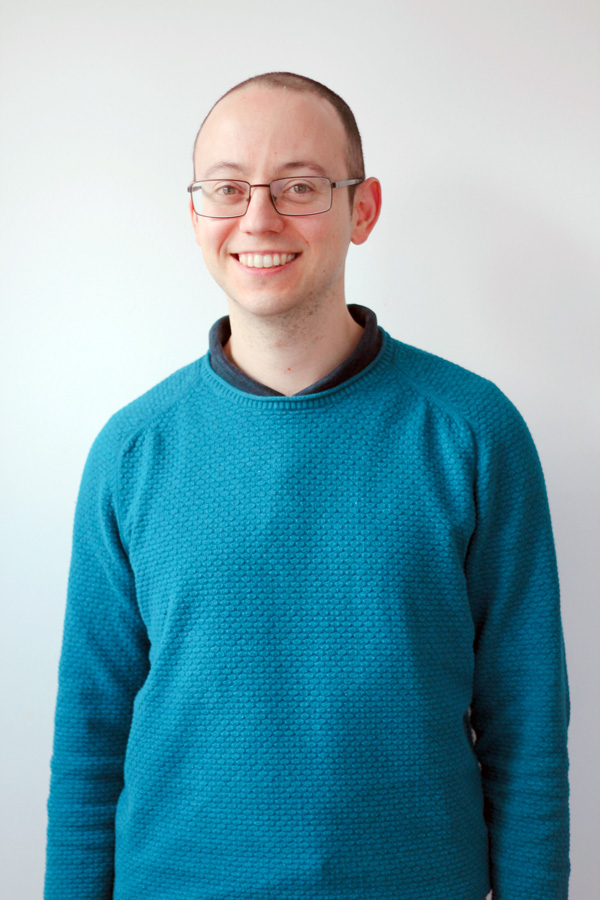
\includegraphics[height=2cm]{graphics/elkouss-david-20211227-torso_0}
%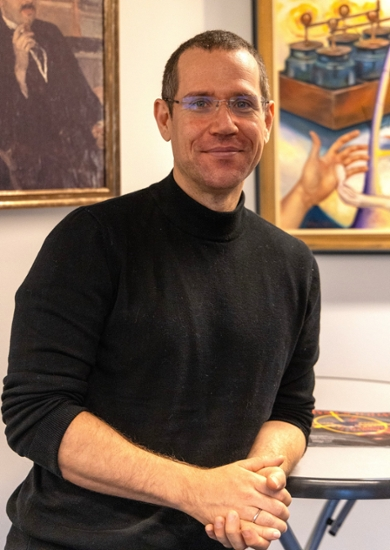
\includegraphics[height=2cm]{graphics/vedran-jobs}
%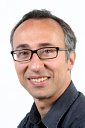
\includegraphics[height=2cm]{graphics/bonsangue}
%
%~~David Elkouss (Okinawa, Delft) ~~~
%Marcello Bonsangue (Leiden)

%\vspace{-2ex}
%Vedran Dunjko (Leiden)


\printbibliography[section=\therefsection]
\end{frame}
\end{refsection}

